\documentclass{scrartcl}

%\usepackage{natbib}
\usepackage{latexrc/macros}

\addbibresource{biblio.bib}

\title{Metastability for the Contact Process on $\integer$}
\author{Owen Lynch \and Kacper Urbański}
\DeclareMathOperator{\expDist}{Exp}

\usepackage{interval}
\newcommand{\ep}{\varepsilon}
\intervalconfig{soft open fences}
\newcommand{\loi}[2]{\interval[open left]{#1}{#2}}
\newcommand{\roi}[2]{\interval[open right]{#1}{#2}}
\newcommand{\Ninf}{\roi{-N}{\infty}}
\newcommand{\infN}{\loi{-\infty}{N}}
\begin{document}

\maketitle
\begin{abstract}
    Metastability is the coexistence of an equilibrium and a ``quasi-equilibrium'' (metastable) state in a system. If we look at a metastable system in time domain, it 
    initially appears to have stabilized in the ``quasi-equilibrium'' state,
    until it suddenly relaxes to the true equilibrium. Metastability is a common phenomenon in nature, with examples ranging from physics to economics and social sciences. 
    This work is a summary of a paper by R. Schonmann \cite{schonmann}, which
    frames this phenomenon as a rigorous property of an abstract interacting particle system - the Contact Process.
\end{abstract}

\section{Overview} \label{overview}

\subsection{Metastability}

Let $\{ \xi_N(t) \}_{N\in\mathbb{N}}$ be a family of Markov processes. The essential idea behind metastability is that, if we were to discretize (``coarse-grain'') time, increasing $N$ would make the process under consideration look more and more like the Markov process in \fref{fig:metastability_nutshell}.

\begin{figure}[h!]
  \centering
  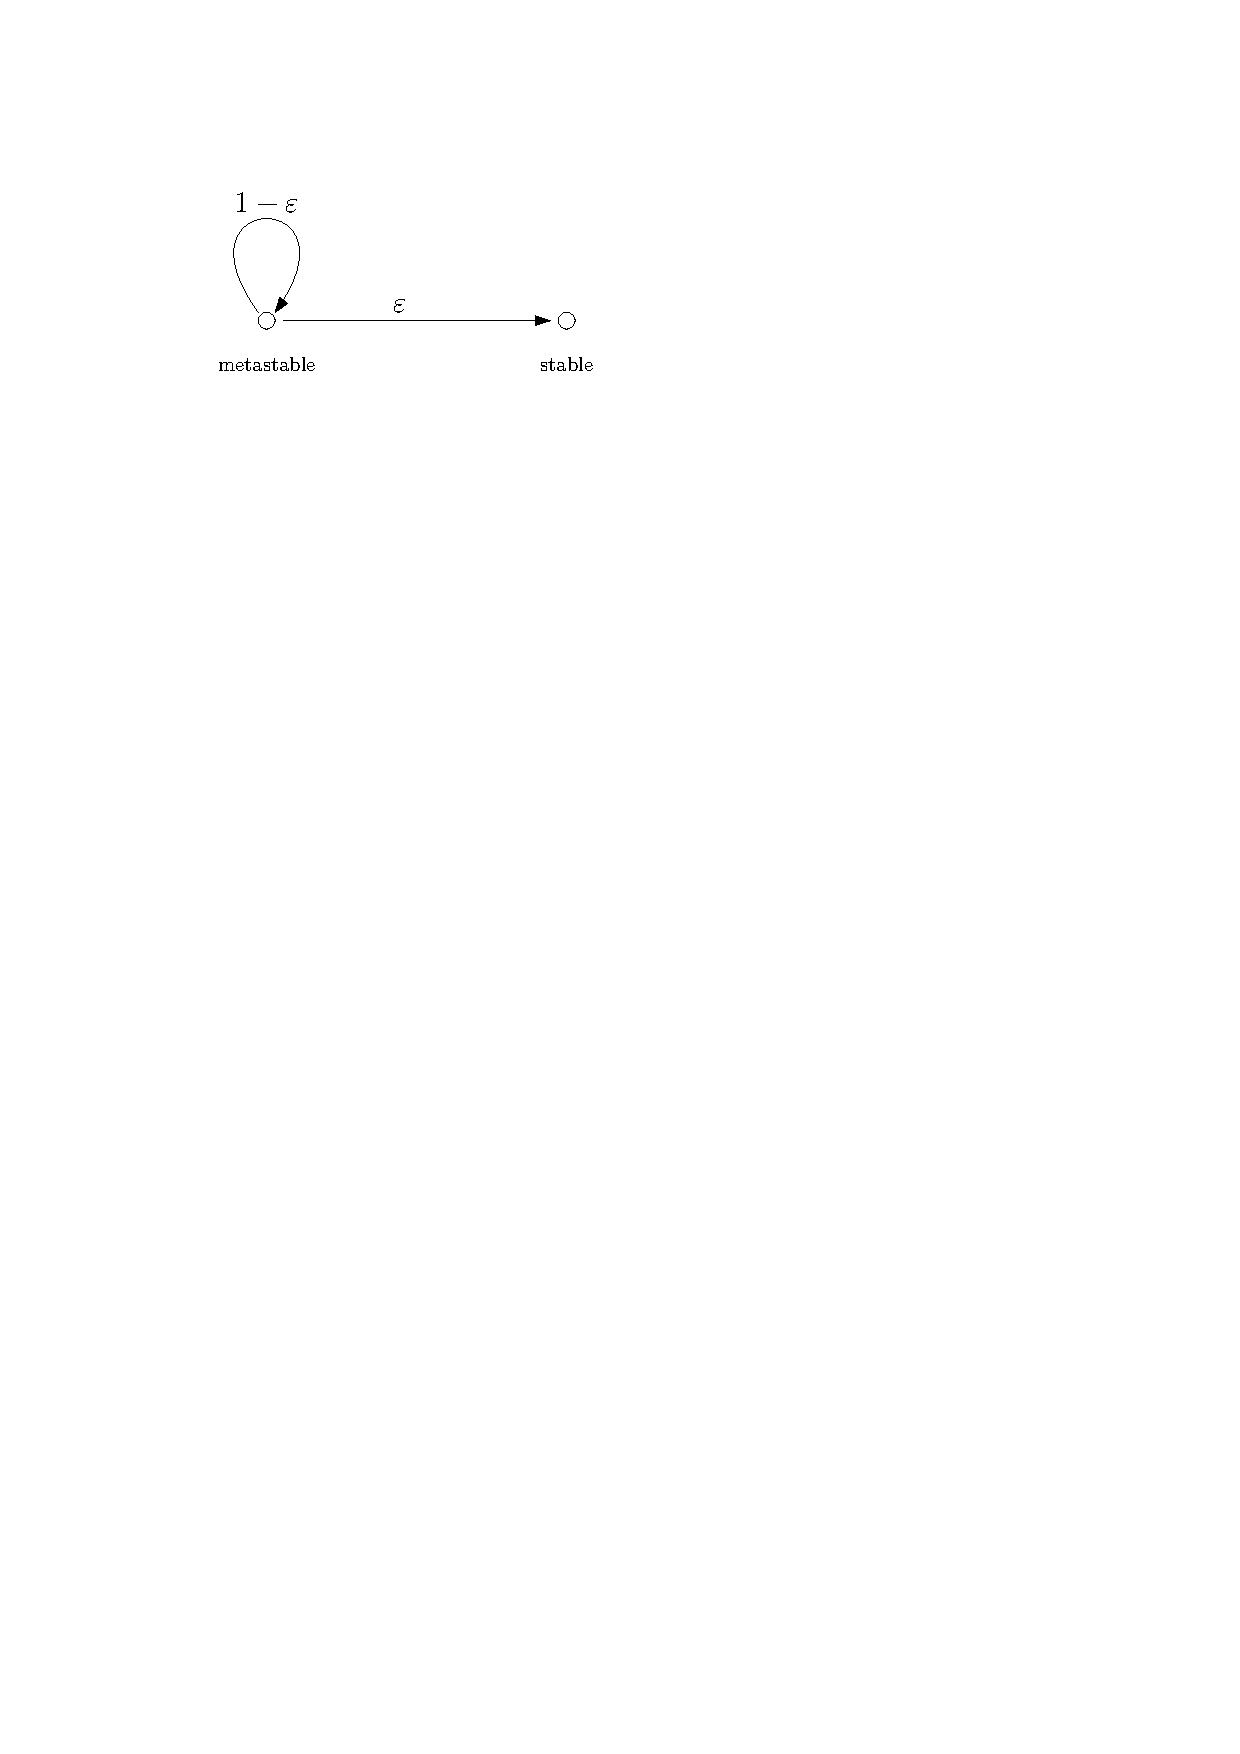
\includegraphics{presentation_owen/metastable_coarse_grain.pdf}
  \caption{Metastability in a Nutshell}
  \label{fig:metastability_nutshell}
\end{figure}

In other words, the system begins in a so-called ``metastable state'', and has a very small chance to move to the stable state at any time. The stable state is either absorbing, or close-to absorbing; in the case that we will talk about in this paper, the stable state is absorbing.

In order to make this ``coarse-graining'' happen, we need two things to be true asymptotically.

\begin{enumerate}
  \item The hitting time of the stable state is exponentially distributed.
  \item Up until the hitting time, temporal means of measurements made to the process converge to an expectation of those measurements with respect to some stationary distribution.
\end{enumerate}

Informally, these two properties allow us to approximate the entire process by sampling from the stationary distribution up until the hitting time, and then putting the system in the absorbing state.

The difficulty comes in stating these two properties precisely. To do this, suppose that $T_{N}$ is the hitting time of the absorbing state, $\mu$ is the stationary distribution, 
and $R_{N}$ is a ``time scale'' parameter that satisfies $R_{N}/\E T_{N} \to 0$. Then we rewrite the two properties more formally as

\begin{enumerate}
  \item $T_{N} / \E T_{N} \to \expDist(1)$ in distribution as $N \to \infty$.
  \item For any $f$ cylindrical,
    \[ \int_{S}^{S + R_{N}} f(\xi_{N}(t)) dt \to \mu(f) \]
    as $N \to \infty$, for any $S + R_{N} < T_{N}$.
\end{enumerate}

This second statement is still very imprecise, and actually mathematically meaningless as currently posed. Also, it turns out that we want a much stronger statement than that. However, we hope that this first statement should ``innoculate'' the reader to the precise statement, which is fairly dense on its own.

\subsection{The Contact Process on $\integer$}

We will use the ``percolation structure'' definition of the contact process, which lends itself better to certain useful constructions.

This ``percolation structure'', consists of for each $x \in \integer$
\begin{enumerate}
  \item A Poisson process $P_{x}$ with rate 1, which we call the ``death'' process at $x$.
  \item A Poisson process $P_{x \to x+1}$ with rate $\lambda$, which we call the ``right infection'' process at $x$.
  \item A Poisson process $P_{x \to x-1}$ with rate $\lambda$, which we call the ``left infection'' process at $x$.
\end{enumerate}

We consider $P_{x}$ to be a random element of $\powerset(\real)$, i.e. $t \in P_{x}$ if and only if the Poisson process ``ticks'' at time $t$.

We define a ``path'' between $(x,s), (y,t) \in \integer \by \real$ with $s \leq t$ to be a sequence
$(z_{0},r_{0}), \ldots, (z_{n},r_{n})$ with $r_{i} \leq r_{i+1}$ such that for all $(z_{i},r_{i}),(z_{i+1},r_{i+1})$, either
\begin{enumerate}
  \item $r_{i} = r_{i+1}$, $\abs{z_{i} - z_{i+1}} = 1$, and $r_{i} \in P_{z_{i} \to z_{i+1}}$. In this case, we are jumping laterally by one line at a time of infection.
  \item $z_{i} = z_{i+1}$, and $[r_{i},r_{i+1}] \cap P_{z_{i}} = \emptyset$. In this case, we are moving along a vertical line, uninterrupted by any deaths.
\end{enumerate}

Define $\xi^{A}(t)$ to be the set of $y$ such that there is a path from $(x,0)$ to $(y,t)$ for some $x \in A$. If the superscript is omitted, then we assume $A = \integer$, i.e. $\xi(t) = \xi^{\integer}(t)$.

For any $A \ins B$, we define $\xi_{B}^{A}(t)$ to be the set of $y$ such that there is a path from $(x,0)$ to $(y,t)$ for some $x \in A$ that stays entirely within $B$. As a special case, we let $\xi_{N}^{A}(t) = \xi_{[-N,N]}^{A}$, for $N \in \natural$. Note that $\xi_{B}$ takes values exclusively in $\powerset(B)$.

One of the most important facts about the contact process is that there is a critical value of $\lambda$, $\lambda_{c}$. For $\lambda < \lambda_{c}$, $\xi(t)$ has a unique extremal invariant measure $\delta_{\emptyset}$. At $\lambda = \lambda_{c}$ the system undergoes a phase transition - for $\lambda > \lambda_{c}$, another extremal invariant measure $\mu$ appears, with the property that
\[ \mu(f) = \limas_{T \to \infty} \frac{1}{T} \int_{0}^{T} \E f(\xi(t)) \dd{t} \]
This measure is not concentrated at $\emptyset$.

For $\xi_{N}(t)$, the only invariant measure is $\delta_{\emptyset}$, because $\emptyset$ is a trap and $\xi_{N}$ takes values on a finite state space. However, as mentioned before, for $\lambda > \lambda_{c}$ an analogue of a phase transition takes place. The system starts being metastable, and stays distributed \emph{approximately} as $\mu$, before a sudden fluctuation takes it to $\emptyset$.

We assume that the reader has a general familiarity with the contact process, and thus we will use some properties later on in the proofs without explicitly discussing them here.

\subsection{Summary}

The object of this paper is to give an overview of the two conditions for metastability for the family of contact processes $\xi_{N}$, in the supercritical regime $\lambda > \lambda_{c}$.

\section{Main Theorems}

\subsection{Exponential Distribution of Hitting Time}

\begin{theorem}[from \cite{schonmann}]
  If $T_{N} = \inf\set{t > 0 \st \xi_{N}(t) \neq \emptyset}$, then
  \[ \frac{T_{N}}{\E T_{N}} \to \expDist(1) \]
  in distribution.
\end{theorem}

To prove this, we first replace $\E T_{N}$ by the unique (by monotonicity) $\beta_{N}$ such that $\Prob(T_{N} > \beta_{N}) = \e^{-1}$. At the end, we will show that $\frac{\E T_{N}}{\beta_{N}} \to 1$.

Let $G_{N}(t) = \Prob[\frac{T_{N}}{\beta_{N}} > t]$, the cumulative distribution function of $T_{N}/\beta_{N}$. Similarly, let $G_{N}^{A}(t) = \Prob[\frac{T^{A}_{N}}{\beta_{N}} > t]$. Note that $G_{N}^{A}(t) \leq G_{N}(t)$ To show that $T_{N}/\beta_{N}$ converges in distribution to $\expDist(1)$, we must show that $G_{N}(t) \to \e^{-t}$. This can be accomplished by showing that
\[ \limas_{N \to \infty} \abs{G_{N}(t+s) - G_{N}(t)G_{N}(s)} = 0 \]
for all $t,s > 0$.

%Note that $G_{N}(t) = \Prob[\xi_{N}(t) \neq \emptyset]$, as $\xi_{N}$ is ``alive'' at time $t$ if and only if $T_{N} > t$. Thus,
%
%\begin{align*}
%  G_{N}(t+s) &= \Prob[\xi_{N}(t+s) \neq \emptyset] \\
%             &= \sum_{A \neq \emptyset} \Prob[\xi_{N}(t+s) \neq \emptyset | \xi_{N}(t) = A] \Prob[\xi_{N}(t) = A] \\
%             &= \sum_{A \neq \emptyset} G_{N}^{A}(s) \Prob[\xi_{N}(t) = A] \\
%             &\leq G_{N}(s) \sum_{A \neq \emptyset} \Prob[\xi_{N}(t) = A] \\
%             &= G_{N}(s) G_{N}(t)
%\end{align*}
%
%Therefore, we are looking to show that $G_{N}(s) G_{N}(t) - G_{N}(t+s) \to 0$ (we can forget the absolute value signs).

It is at this point that we introduce a curious little construction, which seems to not make much sense at first but turns out to be the key to the entire proof. Define $F_{b}$ for $b > 0$ by
\[ F_{b} = \left\{A \ins \integer \st \frac{\abs{A \cap [-b,-1]}}{b} > \frac{\rho}{2}, \frac{\abs{A \cap [1,b]}}{b} > \frac{\rho}{2}\right\} \]
where $\rho = \mu(\set{\eta \st \eta(0) = 1})$.

It is not trivial to show that
\begin{align*}
  \abs{G_{N}(t)G_{N}(s) - G_{N}(t+s)} &\leq \Prob[\xi_{N}(\beta_{N}t) \neq \emptyset] - \min_{A \in F_{b}} \Prob[\xi_{N}^{A}(\beta_{N}t) \neq \emptyset] \\
  &\quad \quad + \Prob[\xi_{N}(\beta_{N}s) \neq \emptyset, \xi_{N}(\beta_{N}s) \notin F_{b}]
\end{align*}
However, the proof is not terribly interesting, and so we refer the reader to Schonman for the details.

The intuition for what this equation is claiming is that we can show that starting in $A \in F_{b}$ is not too different from starting in $[-N,N]$, and we can show that ending \emph{anywhere} non-empty is not too different from ending up somewhere in $F_{b}$. Then a typical process will have probability $G_{N}(t)$ to end up in $A \in F_{b}$ at time $\beta_{N}t$, and then probability $G_{N}(s)$ to end up anywhere non-empty at time $\beta_{N}(t+s)$, starting in some $A \in F_{b}$, so total probability to end up non-empty at time $\beta_{N}(t+s)$ is $G_{N}(t)G_{N}(s)$, as required.

We will have finished if for any $\ep > 0$, we can find $b(\ep)$ and $N(\ep) > b(\ep)$  such that for $N \geq N(\ep)$ and $A \in F_{b}$, we have both
\begin{align}
  \Prob[\xi_{N}(\beta_{N}t) \neq \emptyset] - \Prob[\xi_{N}^{A}(\beta_{N}t) \neq \emptyset] = G_{N}(t) - G_{N}^{A}(t) &< \ep \label{eq:firstineq} \\
  \Prob[\xi_{N}(\beta_{N}s) \neq \emptyset, \xi_{N}(\beta_{N}s) \notin F_{b}] &< \ep \label{eq:secondineq}
\end{align}

We tackle \eref{eq:firstineq} first. Remember that $\xi_{N}(t)$ and $\xi_{N}^{A}$ are defined on the same percolation structure. Therefore, $\xi_{N}(t) \supset \xi_{N}^{A}(t)$, so we have
\[ \Prob[\xi_{N}(\beta_{N} t) \neq \emptyset] - \Prob[\xi_{N}(\beta_{N} t) \neq \emptyset] = \Prob[\xi_{N}(\beta_{N} t) \neq \emptyset, \xi_{N}^{A}(\beta_{N} t) = \emptyset] \leq \Prob[T_{N} \neq T_{N}^{A}] \]

We discussed this proof in the presentation. In short, at a certain time $t$, $\xi_{N}(t) = \xi_{N}^{A}(t) \neq \emptyset$, and by picking $b$ large enough, we can ensure that the process is most likely still alive at this time. Then because of the percolation structure definition, for all $s > t$, $\xi_{N}(s) = \xi_{N}^{A}(s)$, whence $T_{N} = T_{N}^{A}$ with probability greater than $1 - \ep$.

Equation~\ref{eq:secondineq} also relies crucially on the percolation structure. Because of the percolation structure, as long as $\xi_{N}(t) \neq \emptyset$
\[ \xi_{N}(t) = \xi(t) \cap [\min \xi_{N}(t), \max \xi_{N}(t)] \]
To make use of this, we say that $\xi_{N}(t)$ is ``wide'' if $\min \xi_{N}(t) < -N + L$, $\max \xi_{N}(t) > N - L$, for some fixed $L$. Then as long as $[-b,b] \ins [-N+L, N-L]$, for wide $\xi_{N}(t)$, $\xi_{N}(t) \in F_{b}$ if and only if $\xi(t) \in F_{b}$. Now, let $D_{b} = F_{b}^{C} \setminus \set{\emptyset}$.
\begin{align*}
  \Prob[\xi_{N}(\beta_{N}s) \in D_{b}] \leq&\; \Prob[\xi_{N}(\beta_{N}s) \in D_{b}, \min \xi_{N}(\beta_{N}s) < -N + L, \max \xi_{N}(\beta_{N}s) > N - L] \\
                                &+ \Prob[\min \xi_{N}(\beta_{N}s) \geq -N + L, \xi_{N}(\beta_{N}s) \neq \emptyset] \\
                                &+ \Prob[\max \xi_{N}(\beta_{N}s) \leq N - L, \xi_{N}(\beta_{N}s) \neq \emptyset]
\end{align*}
By what we noted earlier, the first term is less than $\Prob(\xi(\beta_{N}s) \in D_{b})$, and we can pick $b$ such that this is less than $\frac{\ep}{3}$.

It remains to minimize the last two terms; by symmetry we only show how to minimize the first. Using a percolation structure argument, it is easy to show that as long as $\xi_{N}(\beta_{N}s) \neq \emptyset$, $\min \xi_{N}(t) = \min \xi_{\Ninf}$. Therefore,
\begin{align*}
  \Prob[\min \xi_{N}(\beta_{N}s) \geq -N + L, \xi_{N}(\beta_{N}) \neq \emptyset] &\geq \Prob[\min \xi_{\Ninf} \geq -N+L] \\
  &\geq \mu_{\Ninf}\set{A \in \Ninf \st A \cap [-N,-N+L-1] = \emptyset}
\end{align*}
We can pick $L$ large enough to make that last term less than $\frac{\ep}{3}$, and we have shown that everything can be made as small as we like, so we are done.

The last thing to do is to show that $\beta_{N}/\E T_{N} \to 1$; this follows from the above proof, as the unique $\beta$ such that $\Prob[\Exp(1) > \beta] = e^{-1}$ is $1 = \E[\Exp(1)]$.

\subsection{Quasi-stationarity up to the Hitting Time}

Recall our initial description of Quasi-stationarity in Section \ref{overview}. To make it more precise, we will define
\begin{description}
    \item[the intermediate timescale] to be a choice of $R_{N} \in \real_{+}$ with $R_{N}/\E[T_{N}] \to 0$
    \item[an observable quantity] to be a cylindrical (local) $f:\{0,1\}^\mathbb{Z} \rightarrow \mathbb{R}$
    \item[the temporal mean] of observable quantity $f$ to be
    \[
        A^N_{R_N}(s, f) := R_N^{-1}\int_s^{s+R_N}f(\xi_N(t))dt
    \]
    \item[the fixed probability distribution] to be $\mu$ (the upper invariant measure of $\xi(t)$)
\end{description}
Note that $A^N_{R_N}$ is a random variable. We will say that this quantity is \emph{close} to $\mu(f)$ if the two converge in probabilty when $N \rightarrow \infty$.

It seems like the definitions given above would be sufficient to make our natural language definition of metastability formal. However, it turns out that an additional technical 
condition is needed. Define
    \[
        \Lambda(f) :=  \text{ smallest } B\subset \mathbb{Z} \text{ s.t. } f(A) = f(A\cap B) \ \forall A \subset \mathbb{Z}
    \]
    Although this is not strictly true, we can think of $\Lambda(f)$ as the ``support'' of $f$.

Our theorem will hold for a specific $L(\varepsilon, f) \in \mathbb{N}$, and we need to have that
\[
    L < N \text{~~and~~} \Lambda(f) \subset [-N+L, N-L]
\]
Notice that $L$ does not depend on $N$. Thus, since we chose to grow $N \rightarrow \infty$, having to choose this $L$ doesn't restrict our choice of $f$ - it merely sets the minimum
 $N$ we can consider.

 We're now ready to give a simplified formulation of what we mean by ``quasi-stationarity''
 \begin{theorem} [from \cite{schonmann}]
        If $\lambda > \lambda^*$ there is a sequence $\{R_N\}_{N \in \mathbb{N}} \subset \mathbb{R_+}$ such that:
        \begin{enumerate}[(a)]
            \item $R_N/\beta_N \rightarrow 0$ as $N\rightarrow \infty$
            \item For all $\varepsilon > 0$ and $f:\{0,1\}^\mathbb{Z} \rightarrow \mathbb{R}$ cylindrical,  $\exists L(\varepsilon, f) \in \mathbb{N}$ such that
                  \[
                      \mathbb{P}\left[ \max_{\mathbb{N}_0 \ni k < K_N}|A_{R_N}(kR_N, f) - \mu(f)| > \varepsilon\right] \rightarrow 0
                  \]
                  as $N \rightarrow \infty$, where $K_N = \max\{k \in \mathbb{N}_0: kR_N < T_N\}$ and $\Lambda(f) \subset [-N + L, N - L] \cap \mathbb{Z}$
        \end{enumerate}
    \end{theorem}

A full proof of this statement is beyond the scope of this article--we will merely give the reader some insight into its key points.

A central claim is that we can make the exceedance probability (given below) arbitrarily small.
\[
    \mathbb{P}\left[ |A_{R_N}(kR_N, f) - \mu(f)| > \varepsilon\right]
\]
We do so in a way which is uniform across all values of $K_N$ and $\mathbb{N}_0 \ni k < K_N$. We estimate this probabilty with a triangle inequality.
\footnotesize
\begin{equation}
    \mathbb{P}\left[ \left|R_N^{-1}\int_{kR_N}^{(k+1)R_N}f(\xi(t))dt - \mu(f)\right| > \varepsilon/2 \right] + 
    \mathbb{P}\left[ \left|R_N^{-1}\int_{kR_N}^{(k+1)R_N}f(\xi_N(t)) - f(\xi(t))dt \right| > \varepsilon/2\right]
    \label{th2:alternative}
\end{equation}
\normalsize
The first term can be made arbitrarily small, as a consequence of $\xi(t) \rightharpoonup \mu(f)$ and exponentially decaying temporal correlations of $\xi(t)$.

To shrink the second term in (\ref{th2:alternative}) we make extensive use of the graphical model construction of the Contact Process. As before, we say $\xi_N(t)$ is \emph{wide} at $t$ if $\min \xi_N(t) < -N + L\ \land\ \max\xi_N(t) > N - L$.
By the fact that we construct all processes on the same percolation structure, and that interactions are between nearest neighbours, we have
\begin{lemma}[Shielding by a wide process]
    If $\xi_N(t)$ is wide at $t$, then \[\xi_N(t) = \xi(t)\text{ on }[-N + L, N - L] \cap \mathbb{Z}\]
    In particular, since $\Lambda(f) \subset [-N+L, N-L]$, we have $f(\xi_N(t)) = f(\xi(t))$
\end{lemma}
Thus, the second term of (\ref{th2:alternative}) will go to 0 if we're able to make it arbitrarily likely for $\xi_N$ to be wide. For any given $N$, it is clear that we can find such an $L$, but we must show that we can find a $L$ that works for all $N$.

To show this, we again make use of the percolation structure. Note that near $-N$, $\xi_N$ will ``look similar'' to $\xi_{\Ninf}$ (this is true as long as $\xi_N$ is alive). By the same reasoning, $\xi_N$ will ``look similar'' to $\xi_{\infN}$ near $N$.
Hence we set $L$ such that
    \[
        \mu_{\Ninf}\left( \left\{ A : A \cap [-N,-N+L] = \varnothing \right\} \right)  \leq \varepsilon/(16\norm{f})
    \]
This makes all possible states of $\xi_N$ that do not intersect $[-N, -N+L]$ very unlikely (by ``looking similar'' to $\xi_{\Ninf}$). By symmetry, this also makes states
that do not intersect $[N-L, N]$ very unlikely. As a final stroke, we use translation invariance to notice that we will get exactly the same effect if we set $L$ 
    \[
        \mu_{\roi{0}{\infty}}\left( \left\{ A : A \cap [0,L] = \varnothing \right\} \right) \leq \varepsilon/(16\norm{f})
    \]
This concludes our overview of the proof of Theorem 2.

\printbibliography
        
\end{document}

